% Options for packages loaded elsewhere
% Options for packages loaded elsewhere
\PassOptionsToPackage{unicode}{hyperref}
\PassOptionsToPackage{hyphens}{url}
%
\documentclass[
  english,
  russian,
  12pt,
  a4paper,
  DIV=11,
  numbers=noendperiod]{scrreprt}
\usepackage{xcolor}
\usepackage{amsmath,amssymb}
\setcounter{secnumdepth}{5}
\usepackage{iftex}
\ifPDFTeX
  \usepackage[T1]{fontenc}
  \usepackage[utf8]{inputenc}
  \usepackage{textcomp} % provide euro and other symbols
\else % if luatex or xetex
  \usepackage{unicode-math} % this also loads fontspec
  \defaultfontfeatures{Scale=MatchLowercase}
  \defaultfontfeatures[\rmfamily]{Ligatures=TeX,Scale=1}
\fi
\usepackage{lmodern}
\ifPDFTeX\else
  % xetex/luatex font selection
\fi
% Use upquote if available, for straight quotes in verbatim environments
\IfFileExists{upquote.sty}{\usepackage{upquote}}{}
\IfFileExists{microtype.sty}{% use microtype if available
  \usepackage[]{microtype}
  \UseMicrotypeSet[protrusion]{basicmath} % disable protrusion for tt fonts
}{}
\usepackage{setspace}
% Make \paragraph and \subparagraph free-standing
\makeatletter
\ifx\paragraph\undefined\else
  \let\oldparagraph\paragraph
  \renewcommand{\paragraph}{
    \@ifstar
      \xxxParagraphStar
      \xxxParagraphNoStar
  }
  \newcommand{\xxxParagraphStar}[1]{\oldparagraph*{#1}\mbox{}}
  \newcommand{\xxxParagraphNoStar}[1]{\oldparagraph{#1}\mbox{}}
\fi
\ifx\subparagraph\undefined\else
  \let\oldsubparagraph\subparagraph
  \renewcommand{\subparagraph}{
    \@ifstar
      \xxxSubParagraphStar
      \xxxSubParagraphNoStar
  }
  \newcommand{\xxxSubParagraphStar}[1]{\oldsubparagraph*{#1}\mbox{}}
  \newcommand{\xxxSubParagraphNoStar}[1]{\oldsubparagraph{#1}\mbox{}}
\fi
\makeatother


\usepackage{longtable,booktabs,array}
\usepackage{calc} % for calculating minipage widths
% Correct order of tables after \paragraph or \subparagraph
\usepackage{etoolbox}
\makeatletter
\patchcmd\longtable{\par}{\if@noskipsec\mbox{}\fi\par}{}{}
\makeatother
% Allow footnotes in longtable head/foot
\IfFileExists{footnotehyper.sty}{\usepackage{footnotehyper}}{\usepackage{footnote}}
\makesavenoteenv{longtable}
\usepackage{graphicx}
\makeatletter
\newsavebox\pandoc@box
\newcommand*\pandocbounded[1]{% scales image to fit in text height/width
  \sbox\pandoc@box{#1}%
  \Gscale@div\@tempa{\textheight}{\dimexpr\ht\pandoc@box+\dp\pandoc@box\relax}%
  \Gscale@div\@tempb{\linewidth}{\wd\pandoc@box}%
  \ifdim\@tempb\p@<\@tempa\p@\let\@tempa\@tempb\fi% select the smaller of both
  \ifdim\@tempa\p@<\p@\scalebox{\@tempa}{\usebox\pandoc@box}%
  \else\usebox{\pandoc@box}%
  \fi%
}
% Set default figure placement to htbp
\def\fps@figure{htbp}
\makeatother



\ifLuaTeX
\usepackage[bidi=basic,provide=*]{babel}
\else
\usepackage[bidi=default,provide=*]{babel}
\fi
% get rid of language-specific shorthands (see #6817):
\let\LanguageShortHands\languageshorthands
\def\languageshorthands#1{}


\setlength{\emergencystretch}{3em} % prevent overfull lines

\providecommand{\tightlist}{%
  \setlength{\itemsep}{0pt}\setlength{\parskip}{0pt}}



 
\usepackage[style=gost-numeric,backend=biber,langhook=extras,autolang=other*]{biblatex}
\addbibresource{bib/cite.bib}

\usepackage[]{csquotes}

\usepackage{indentfirst}
\usepackage{float}
\floatplacement{figure}{H}
\IfFileExists{plex-otf.sty}{
  %% Full TeXlive
  \usepackage[
    % math,
    RM={Scale=0.94},SS={Scale=0.94},SScon={Scale=0.94},TT={Scale=MatchLowercase,FakeStretch=0.9},
    DefaultFeatures={Ligatures=Common}
  ]{plex-otf}
  % \usepackage[Scale=MatchUppercase]{juliamono}
}{
  %% TinyTeX
  \usepackage{libertine}
}
\KOMAoption{captions}{tableheading}
\makeatletter
\@ifpackageloaded{caption}{}{\usepackage{caption}}
\AtBeginDocument{%
\ifdefined\contentsname
  \renewcommand*\contentsname{Содержание}
\else
  \newcommand\contentsname{Содержание}
\fi
\ifdefined\listfigurename
  \renewcommand*\listfigurename{Список иллюстраций}
\else
  \newcommand\listfigurename{Список иллюстраций}
\fi
\ifdefined\listtablename
  \renewcommand*\listtablename{Список таблиц}
\else
  \newcommand\listtablename{Список таблиц}
\fi
\ifdefined\figurename
  \renewcommand*\figurename{Рисунок}
\else
  \newcommand\figurename{Рисунок}
\fi
\ifdefined\tablename
  \renewcommand*\tablename{Таблица}
\else
  \newcommand\tablename{Таблица}
\fi
}
\@ifpackageloaded{float}{}{\usepackage{float}}
\floatstyle{ruled}
\@ifundefined{c@chapter}{\newfloat{codelisting}{h}{lop}}{\newfloat{codelisting}{h}{lop}[chapter]}
\floatname{codelisting}{Список}
\newcommand*\listoflistings{\listof{codelisting}{Листинги}}
\makeatother
\makeatletter
\makeatother
\makeatletter
\@ifpackageloaded{caption}{}{\usepackage{caption}}
\@ifpackageloaded{subcaption}{}{\usepackage{subcaption}}
\makeatother
\usepackage{bookmark}
\IfFileExists{xurl.sty}{\usepackage{xurl}}{} % add URL line breaks if available
\urlstyle{same}
\hypersetup{
  pdftitle={Отчёт по лабораторной работе №3},
  pdfauthor={Самарханова Полина Тимуровна},
  pdflang={ru-RU},
  hidelinks,
  pdfcreator={LaTeX via pandoc}}


\title{Отчёт по лабораторной работе №3}
\usepackage{etoolbox}
\makeatletter
\providecommand{\subtitle}[1]{% add subtitle to \maketitle
  \apptocmd{\@title}{\par {\large #1 \par}}{}{}
}
\makeatother
\subtitle{Имитационное моделирование}
\author{Самарханова Полина Тимуровна}
\date{}
\begin{document}
\maketitle

\renewcommand*\contentsname{Содержание}
{
\setcounter{tocdepth}{1}
\tableofcontents
}
\listoffigures
\listoftables

\setstretch{1.5}
\chapter{Цель
работы}\label{ux446ux435ux43bux44c-ux440ux430ux431ux43eux442ux44b}

Целью данной лабораторной работы является освоение методологии агентного
моделирования (Agent-Based Modeling, ABM) на примере модели Daisyworld,
а также приобретение практических навыков разработки, визуализации и
анализа агентных моделей с использованием пакета Agents.jl в среде
Julia.

\chapter{Задание}\label{ux437ux430ux434ux430ux43dux438ux435}

\begin{itemize}
\tightlist
\item
  Создать рабочий каталог для всего курса. -Установить необходимые
  пакеты.
\item
  Выполнить предложенный код.
\item
  Преобразовать код в литературный стиль.
\item
  Сгенерировать из литературного кода:

  \begin{itemize}
  \tightlist
  \item
    чистый код;
  \item
    jupyter notebook;
  \item
    документацию в формате Quarto.
  \end{itemize}
\item
  Выполнить код из jupyter notebook.
\item
  Интегрировать документацию в формате Quarto в отчёт.
\item
  Добавить в код в литературном стиле вычисление для набора параметров.
\item
  Сгенерировать из литературного кода с параметрами:

  \begin{itemize}
  \tightlist
  \item
    чистый код;
  \item
    jupyter notebook;
  \item
    документацию в формате Quarto.
  \end{itemize}
\item
  Выполнить код из jupyter notebook с параметрами.
\item
  Интегрировать документацию с параметрами в формате Quarto в отчёт.
\end{itemize}

\chapter{Выполнение лабораторной
работы}\label{ux432ux44bux43fux43eux43bux43dux435ux43dux438ux435-ux43bux430ux431ux43eux440ux430ux442ux43eux440ux43dux43eux439-ux440ux430ux431ux43eux442ux44b}

\section{Реализация на
Agents.jl}\label{ux440ux435ux430ux43bux438ux437ux430ux446ux438ux44f-ux43dux430-agents.jl}

Перехожу в каталог лабораторной работы 3 и создаю папку scr и файл
daisyworld.jl (рис.~\ref{fig-1}).

\begin{figure}

\centering{


\includegraphics[width=0.7\linewidth,height=\textheight,keepaspectratio]{image/1.png}

}

\caption{\label{fig-1}создание файла}

\end{figure}%

В открывшемся окне вставила код из методички (рис.~\ref{fig-2}).

\begin{figure}

\centering{


\includegraphics[width=0.7\linewidth,height=\textheight,keepaspectratio]{image/2.png}

}

\caption{\label{fig-2}код}

\end{figure}%

Установила необходимые пакеты (рис.~\ref{fig-3}).

\begin{figure}

\centering{


\includegraphics[width=0.7\linewidth,height=\textheight,keepaspectratio]{image/3.png}

}

\caption{\label{fig-3}установка пакетов}

\end{figure}%

Подключила файл с моделью (рис.~\ref{fig-4}).

\begin{figure}

\centering{


\includegraphics[width=0.7\linewidth,height=\textheight,keepaspectratio]{image/4.png}

}

\caption{\label{fig-4}подключение}

\end{figure}%

Создала модель(рис.~\ref{fig-5}).

\begin{figure}

\centering{


\includegraphics[width=0.7\linewidth,height=\textheight,keepaspectratio]{image/5.png}

}

\caption{\label{fig-5}модель}

\end{figure}%

Запустила программу и получил результат (рис.~\ref{fig-6}).

\begin{figure}

\centering{


\includegraphics[width=0.7\linewidth,height=\textheight,keepaspectratio]{image/6.png}

}

\caption{\label{fig-6}результат}

\end{figure}%

\section{Базовая
визуализация}\label{ux431ux430ux437ux43eux432ux430ux44f-ux432ux438ux437ux443ux430ux43bux438ux437ux430ux446ux438ux44f}

Установила необходимые пакеты (рис.~\ref{fig-7}).

\begin{figure}

\centering{


\includegraphics[width=0.7\linewidth,height=\textheight,keepaspectratio]{image/7.png}

}

\caption{\label{fig-7}установка пакетов}

\end{figure}%

Создала файл scripts/daisyworld.jl (рис.~\ref{fig-8}).

\begin{figure}

\centering{


\includegraphics[width=0.7\linewidth,height=\textheight,keepaspectratio]{image/8.png}

}

\caption{\label{fig-8}файл}

\end{figure}%

В открывшемся окне вставила код из медодички (рис.~\ref{fig-9}).

\begin{figure}

\centering{


\includegraphics[width=0.7\linewidth,height=\textheight,keepaspectratio]{image/9.png}

}

\caption{\label{fig-9}код}

\end{figure}%

Запустила код(рис.~\ref{fig-10}).

\begin{figure}

\centering{


\includegraphics[width=0.7\linewidth,height=\textheight,keepaspectratio]{image/10.png}

}

\caption{\label{fig-10}запуск}

\end{figure}%

Посмотрела результат (рис.~\ref{fig-11}).

\begin{figure}

\centering{


\includegraphics[width=0.7\linewidth,height=\textheight,keepaspectratio]{image/11.png}

}

\caption{\label{fig-11}графики}

\end{figure}%

Открыла файл для литературного кода(рис.~\ref{fig-14}).

\begin{figure}

\centering{


\includegraphics[width=0.7\linewidth,height=\textheight,keepaspectratio]{image/14.png}

}

\caption{\label{fig-14}файл}

\end{figure}%

В открывшеся окне вставила литературный код (рис.~\ref{fig-15}).

\begin{figure}

\centering{


\includegraphics[width=0.7\linewidth,height=\textheight,keepaspectratio]{image/15.png}

}

\caption{\label{fig-15}запуск LV}

\end{figure}%

Сгенерировала чистый код (рис.~\ref{fig-16}).

\begin{figure}

\centering{


\includegraphics[width=0.7\linewidth,height=\textheight,keepaspectratio]{image/16.png}

}

\caption{\label{fig-16}генерируем чистый код}

\end{figure}%

Запустила код из юпитера(рис.~\ref{fig-17}).

\begin{figure}

\centering{


\includegraphics[width=0.7\linewidth,height=\textheight,keepaspectratio]{image/17.png}

}

\caption{\label{fig-17}запуск кода из юпитера}

\end{figure}%

\section{Анимация
модели}\label{ux430ux43dux438ux43cux430ux446ux438ux44f-ux43cux43eux434ux435ux43bux438}

Установила необходимые пакеты (\textbf{?@fig-18}).

\begin{figure}

\centering{


\includegraphics[width=0.7\linewidth,height=\textheight,keepaspectratio]{image/19.png}

}

\caption{\label{fig-19}файл}

\end{figure}%

В открывшемся окне вставила код из медодички (рис.~\ref{fig-20}).

\begin{figure}

\centering{

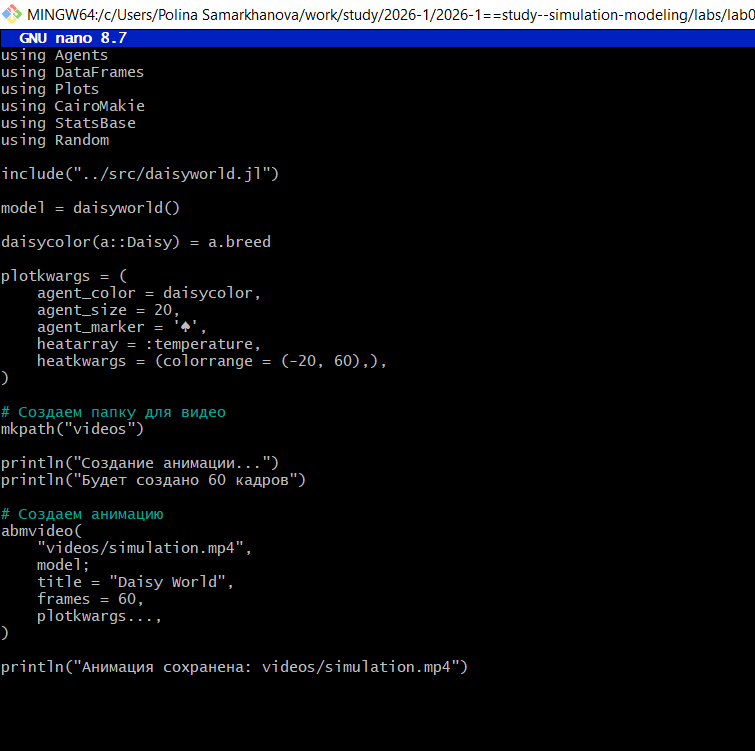
\includegraphics[width=0.7\linewidth,height=\textheight,keepaspectratio]{image/20.png}

}

\caption{\label{fig-20}код}

\end{figure}%

Запустила код, видео выложила на платформы (рис.~\ref{fig-21}).

\begin{figure}

\centering{

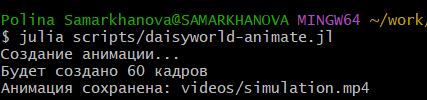
\includegraphics[width=0.7\linewidth,height=\textheight,keepaspectratio]{image/21.png}

}

\caption{\label{fig-21}запуск}

\end{figure}%

\section{Динамика числа
маргариток}\label{ux434ux438ux43dux430ux43cux438ux43aux430-ux447ux438ux441ux43bux430-ux43cux430ux440ux433ux430ux440ux438ux442ux43eux43a}

Создала файл scripts/daisyworld-count.jl (рис.~\ref{fig-22}).

\begin{figure}

\centering{

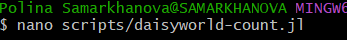
\includegraphics[width=0.7\linewidth,height=\textheight,keepaspectratio]{image/22.png}

}

\caption{\label{fig-22}файл}

\end{figure}%

В открывшемся окне вставила код из медодички (рис.~\ref{fig-23}).

\begin{figure}

\centering{

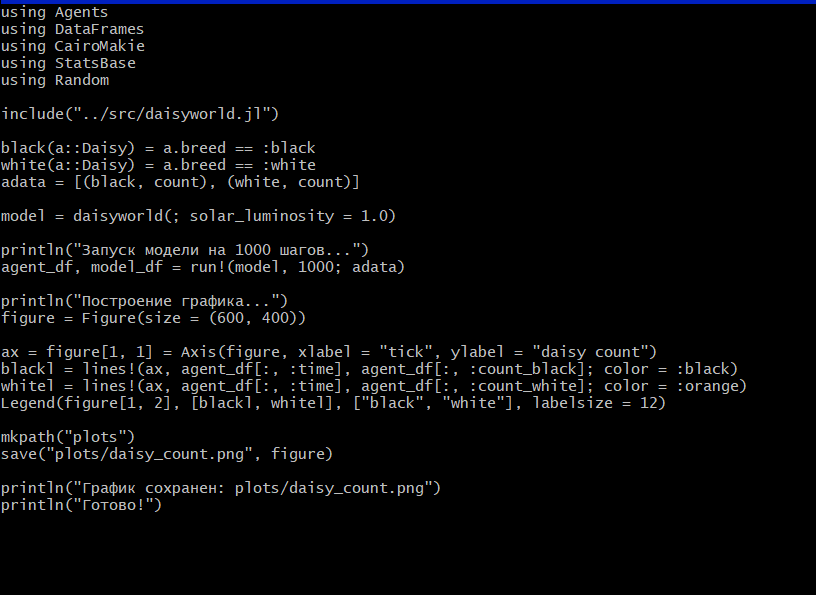
\includegraphics[width=0.7\linewidth,height=\textheight,keepaspectratio]{image/23.png}

}

\caption{\label{fig-23}код}

\end{figure}%

Запустила код(рис.~\ref{fig-24}).

\begin{figure}

\centering{

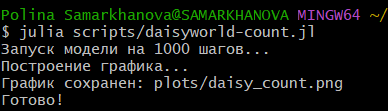
\includegraphics[width=0.7\linewidth,height=\textheight,keepaspectratio]{image/24.png}

}

\caption{\label{fig-24}запуск}

\end{figure}%

Посмотрела результат (рис.~\ref{fig-25}).

\begin{figure}

\centering{

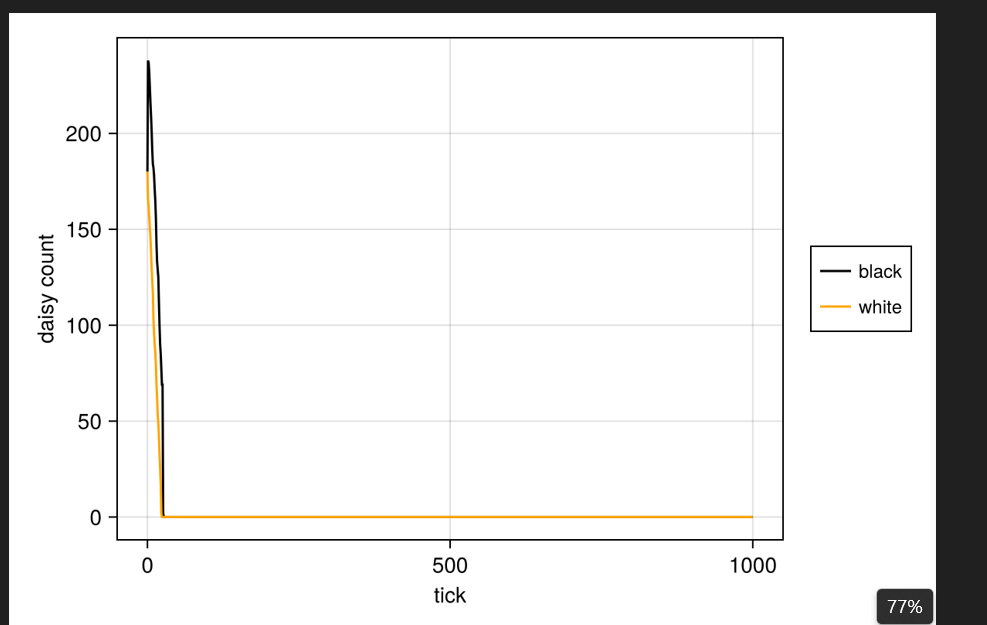
\includegraphics[width=0.7\linewidth,height=\textheight,keepaspectratio]{image/25.png}

}

\caption{\label{fig-25}графики}

\end{figure}%

\section{Динамика
модели}\label{ux434ux438ux43dux430ux43cux438ux43aux430-ux43cux43eux434ux435ux43bux438}

Создала файл scripts/daisyworld-luminosity.jl (рис.~\ref{fig-26}).

\begin{figure}

\centering{

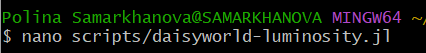
\includegraphics[width=0.7\linewidth,height=\textheight,keepaspectratio]{image/26.png}

}

\caption{\label{fig-26}файл}

\end{figure}%

В открывшемся окне вставила код из медодички (рис.~\ref{fig-27}).

\begin{figure}

\centering{

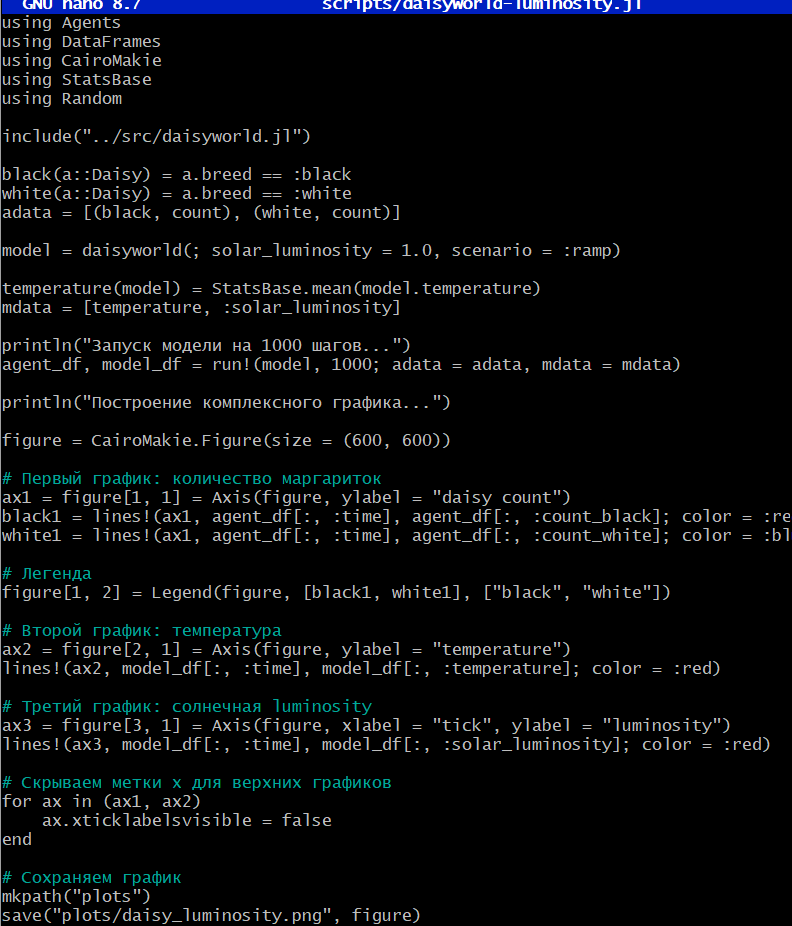
\includegraphics[width=0.7\linewidth,height=\textheight,keepaspectratio]{image/27.png}

}

\caption{\label{fig-27}код}

\end{figure}%

Запустила код(рис.~\ref{fig-28}).

\begin{figure}

\centering{

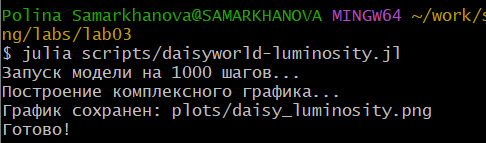
\includegraphics[width=0.7\linewidth,height=\textheight,keepaspectratio]{image/28.png}

}

\caption{\label{fig-28}запуск}

\end{figure}%

Посмотрела результат (рис.~\ref{fig-29}).

\begin{figure}

\centering{

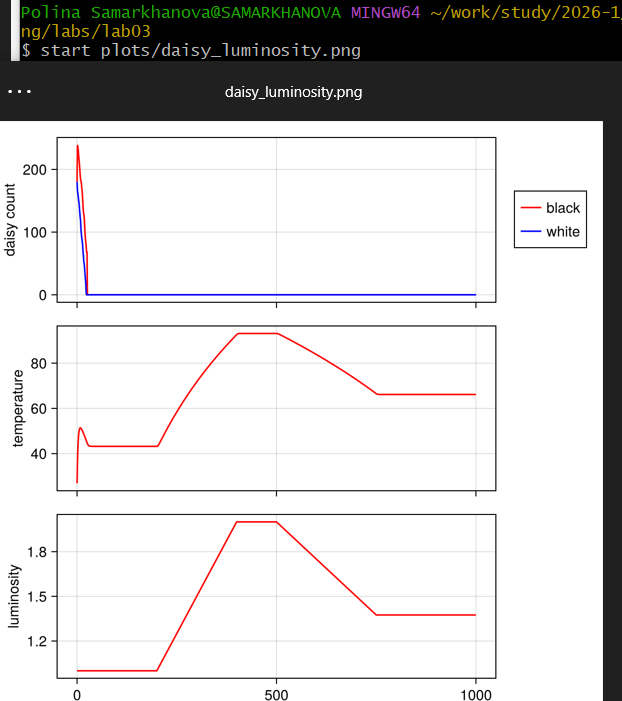
\includegraphics[width=0.7\linewidth,height=\textheight,keepaspectratio]{image/29.png}

}

\caption{\label{fig-29}графики}

\end{figure}%

\section{Базовая
визуализация(параметры)}\label{ux431ux430ux437ux43eux432ux430ux44f-ux432ux438ux437ux443ux430ux43bux438ux437ux430ux446ux438ux44fux43fux430ux440ux430ux43cux435ux442ux440ux44b}

Создала файл scripts/daisyworld\_param.jl (рис.~\ref{fig-30}).

\begin{figure}

\centering{

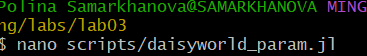
\includegraphics[width=0.7\linewidth,height=\textheight,keepaspectratio]{image/30.png}

}

\caption{\label{fig-30}файл}

\end{figure}%

В открывшемся окне вставила код из медодички (рис.~\ref{fig-31}).

\begin{figure}

\centering{

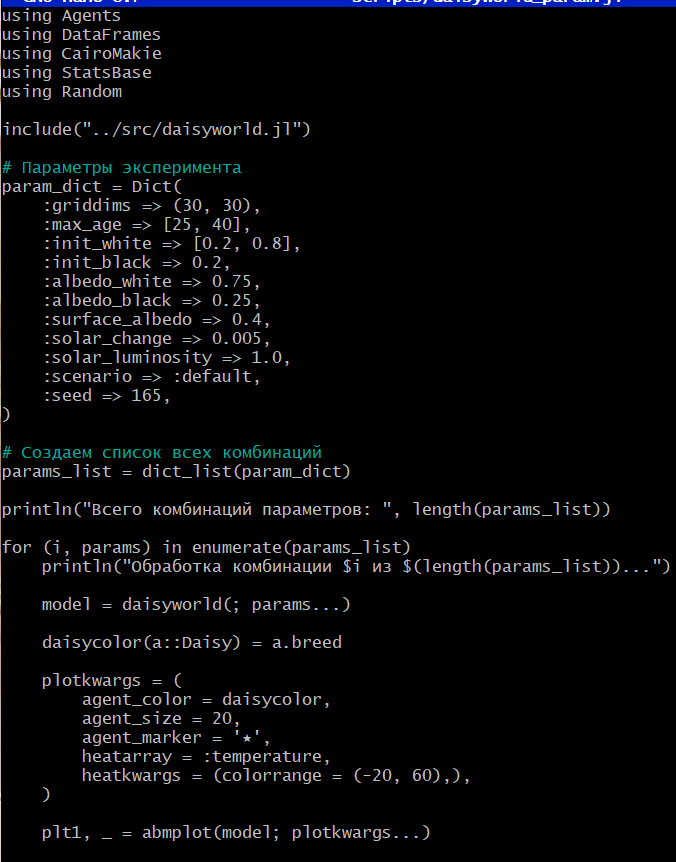
\includegraphics[width=0.7\linewidth,height=\textheight,keepaspectratio]{image/31.png}

}

\caption{\label{fig-31}код}

\end{figure}%

Запустила код(рис.~\ref{fig-32}).

\begin{figure}

\centering{

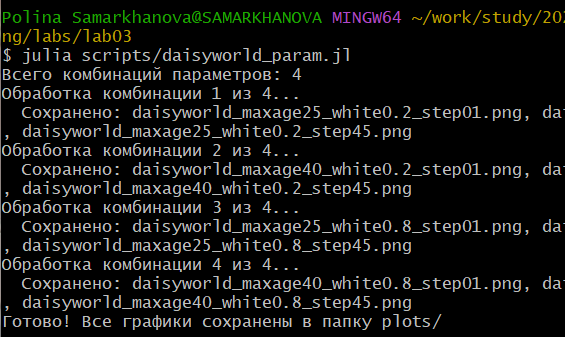
\includegraphics[width=0.7\linewidth,height=\textheight,keepaspectratio]{image/32.png}

}

\caption{\label{fig-32}запуск}

\end{figure}%

Посмотрела результат (рис.~\ref{fig-33}).

\begin{figure}

\centering{

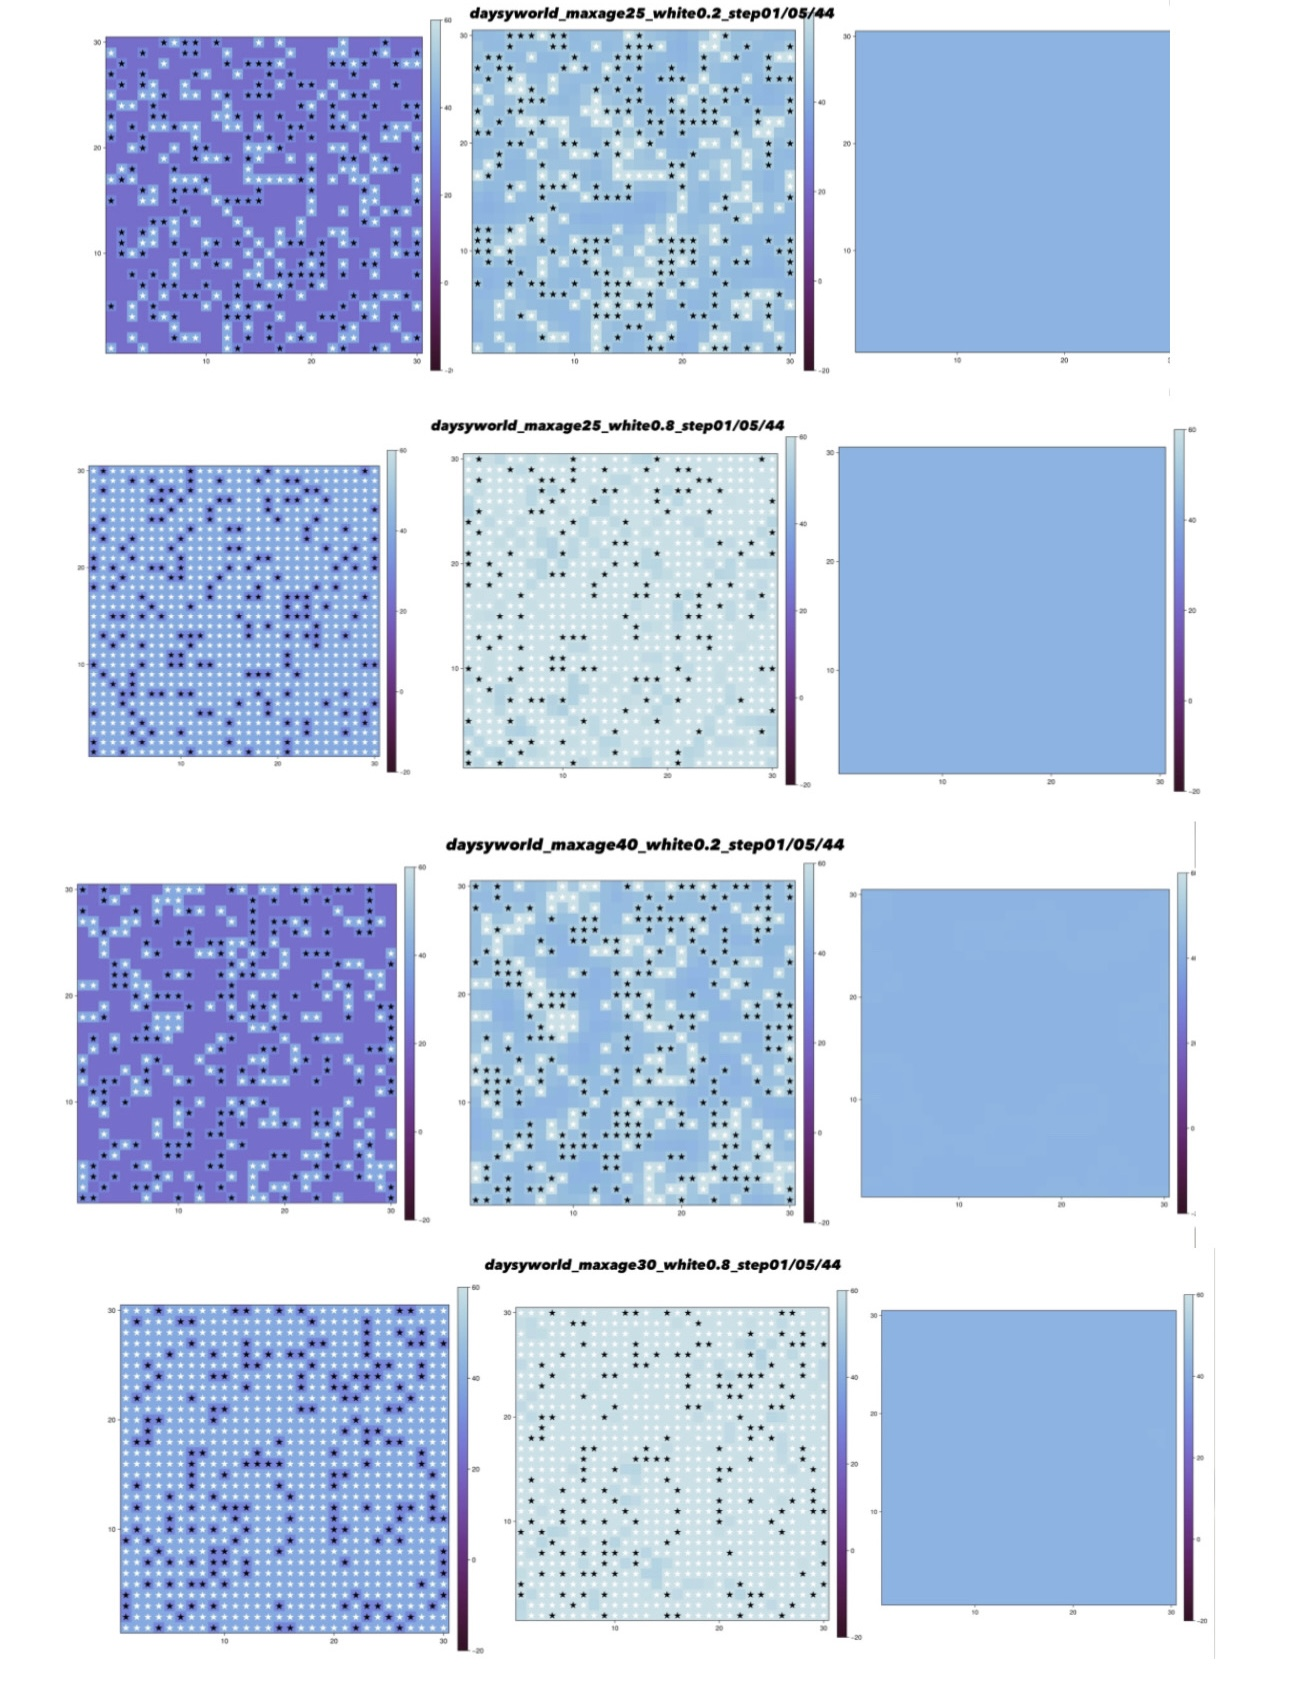
\includegraphics[width=0.7\linewidth,height=\textheight,keepaspectratio]{image/33.png}

}

\caption{\label{fig-33}графики}

\end{figure}%

\section{Динамика числа
маргариток(параметры)}\label{ux434ux438ux43dux430ux43cux438ux43aux430-ux447ux438ux441ux43bux430-ux43cux430ux440ux433ux430ux440ux438ux442ux43eux43aux43fux430ux440ux430ux43cux435ux442ux440ux44b}

Создала файл scripts/daisyworld-count\_param.jl (рис.~\ref{fig-34}).

\begin{figure}

\centering{

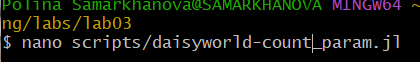
\includegraphics[width=0.7\linewidth,height=\textheight,keepaspectratio]{image/34.png}

}

\caption{\label{fig-34}файл}

\end{figure}%

В открывшемся окне вставила код из медодички (рис.~\ref{fig-35}).

\begin{figure}

\centering{

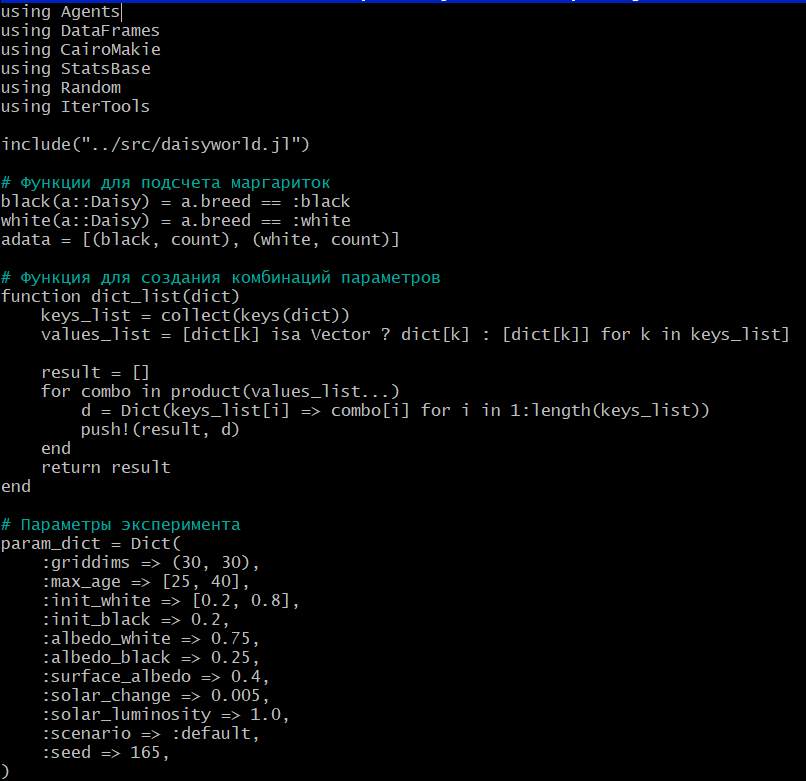
\includegraphics[width=0.7\linewidth,height=\textheight,keepaspectratio]{image/35.png}

}

\caption{\label{fig-35}код}

\end{figure}%

Запустила код(рис.~\ref{fig-36}).

\begin{figure}

\centering{

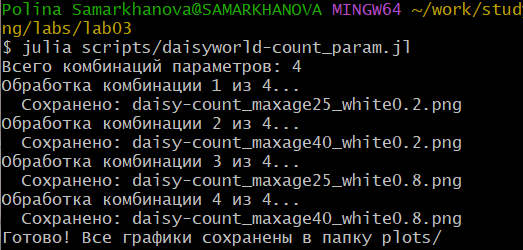
\includegraphics[width=0.7\linewidth,height=\textheight,keepaspectratio]{image/36.png}

}

\caption{\label{fig-36}запуск}

\end{figure}%

Посмотрела результат (рис.~\ref{fig-37}).

\begin{figure}

\centering{

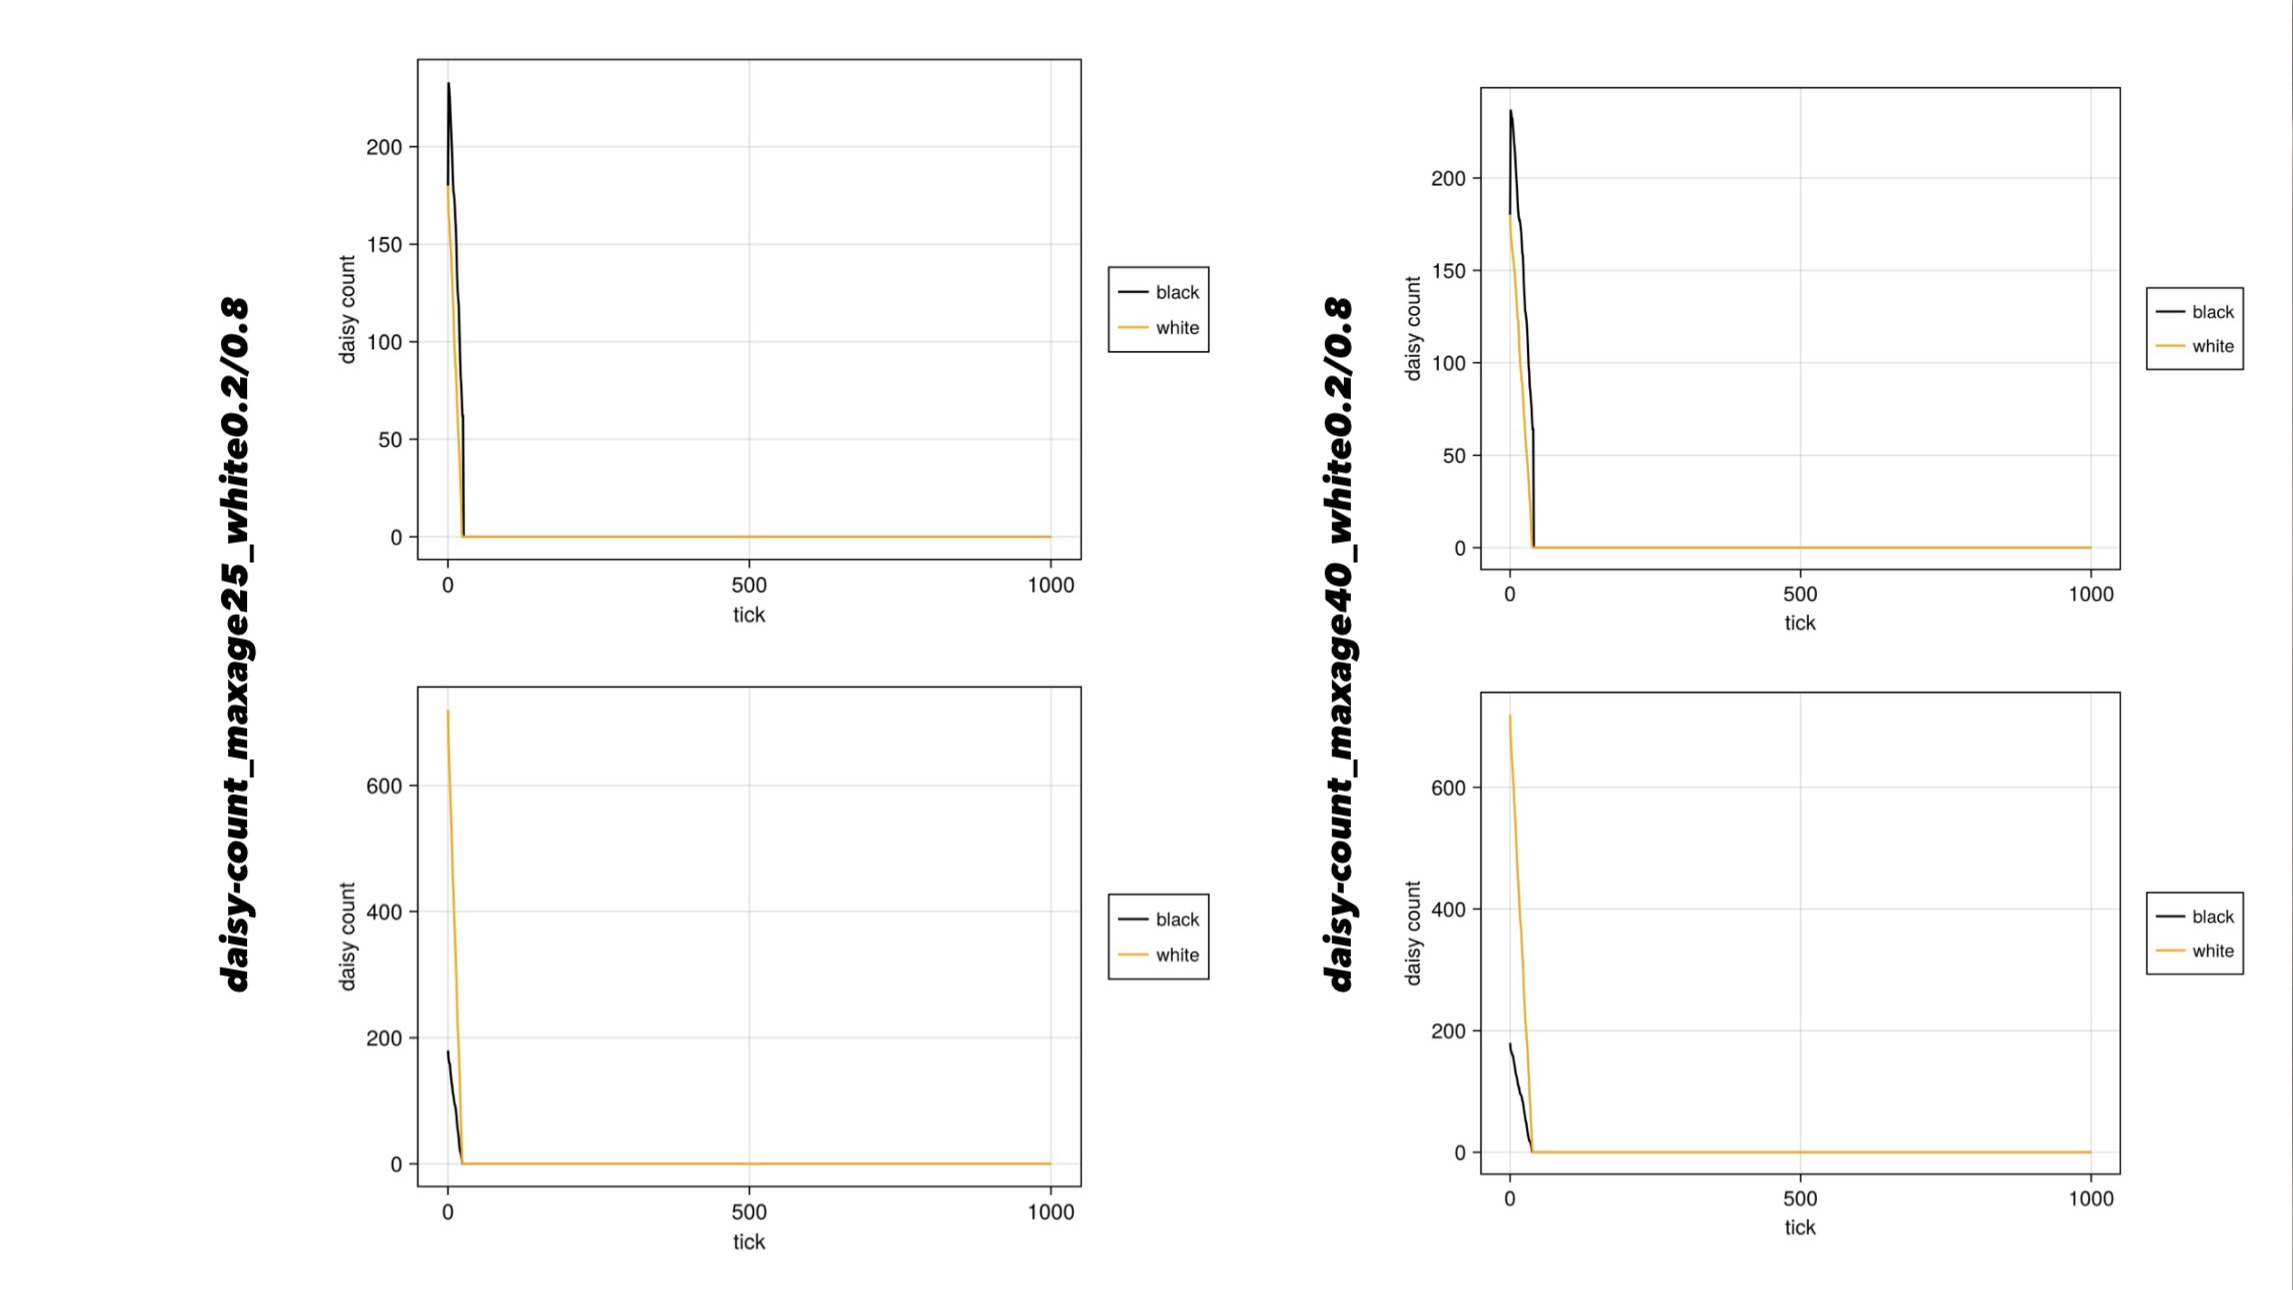
\includegraphics[width=0.7\linewidth,height=\textheight,keepaspectratio]{image/37.png}

}

\caption{\label{fig-37}графики}

\end{figure}%

\section{Динамика
модели(параметры)}\label{ux434ux438ux43dux430ux43cux438ux43aux430-ux43cux43eux434ux435ux43bux438ux43fux430ux440ux430ux43cux435ux442ux440ux44b}

Создала файл scripts/daisyworld-luminosity\_param.jl
(рис.~\ref{fig-38}).

\begin{figure}

\centering{

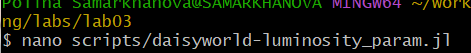
\includegraphics[width=0.7\linewidth,height=\textheight,keepaspectratio]{image/38.png}

}

\caption{\label{fig-38}файл}

\end{figure}%

В открывшемся окне вставила код из медодички (рис.~\ref{fig-39}).

\begin{figure}

\centering{

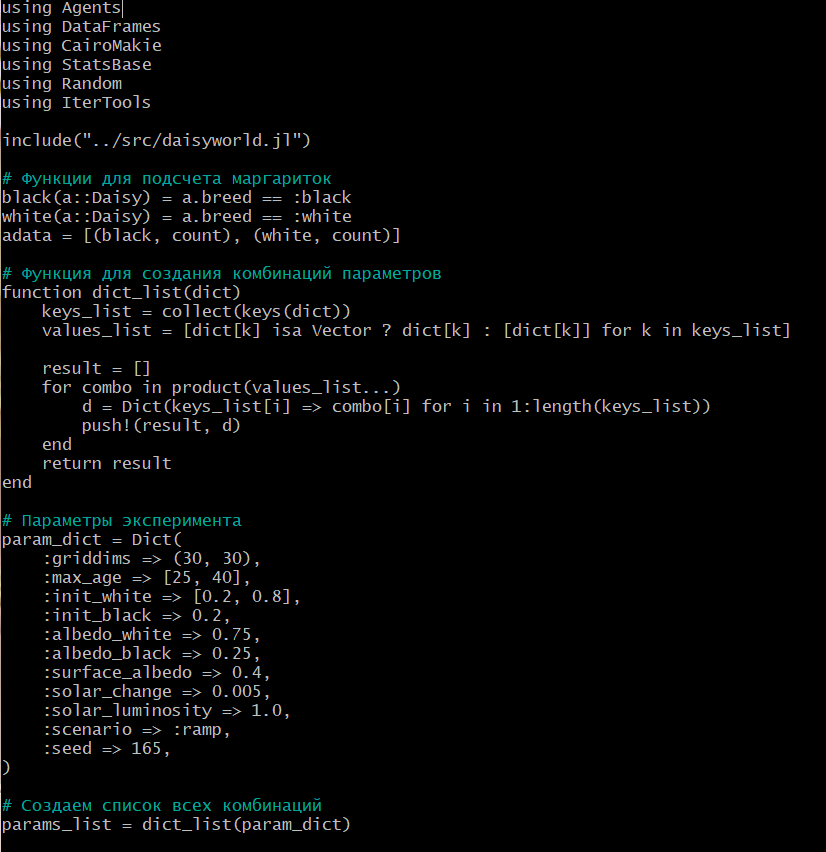
\includegraphics[width=0.7\linewidth,height=\textheight,keepaspectratio]{image/39.png}

}

\caption{\label{fig-39}код}

\end{figure}%

Запустила код(рис.~\ref{fig-40}).

\begin{figure}

\centering{

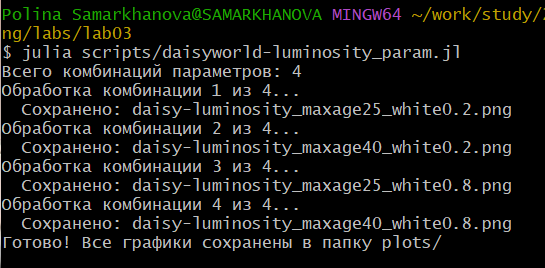
\includegraphics[width=0.7\linewidth,height=\textheight,keepaspectratio]{image/40.png}

}

\caption{\label{fig-40}запуск}

\end{figure}%

Посмотрела результат (рис.~\ref{fig-41}).

\begin{figure}

\centering{

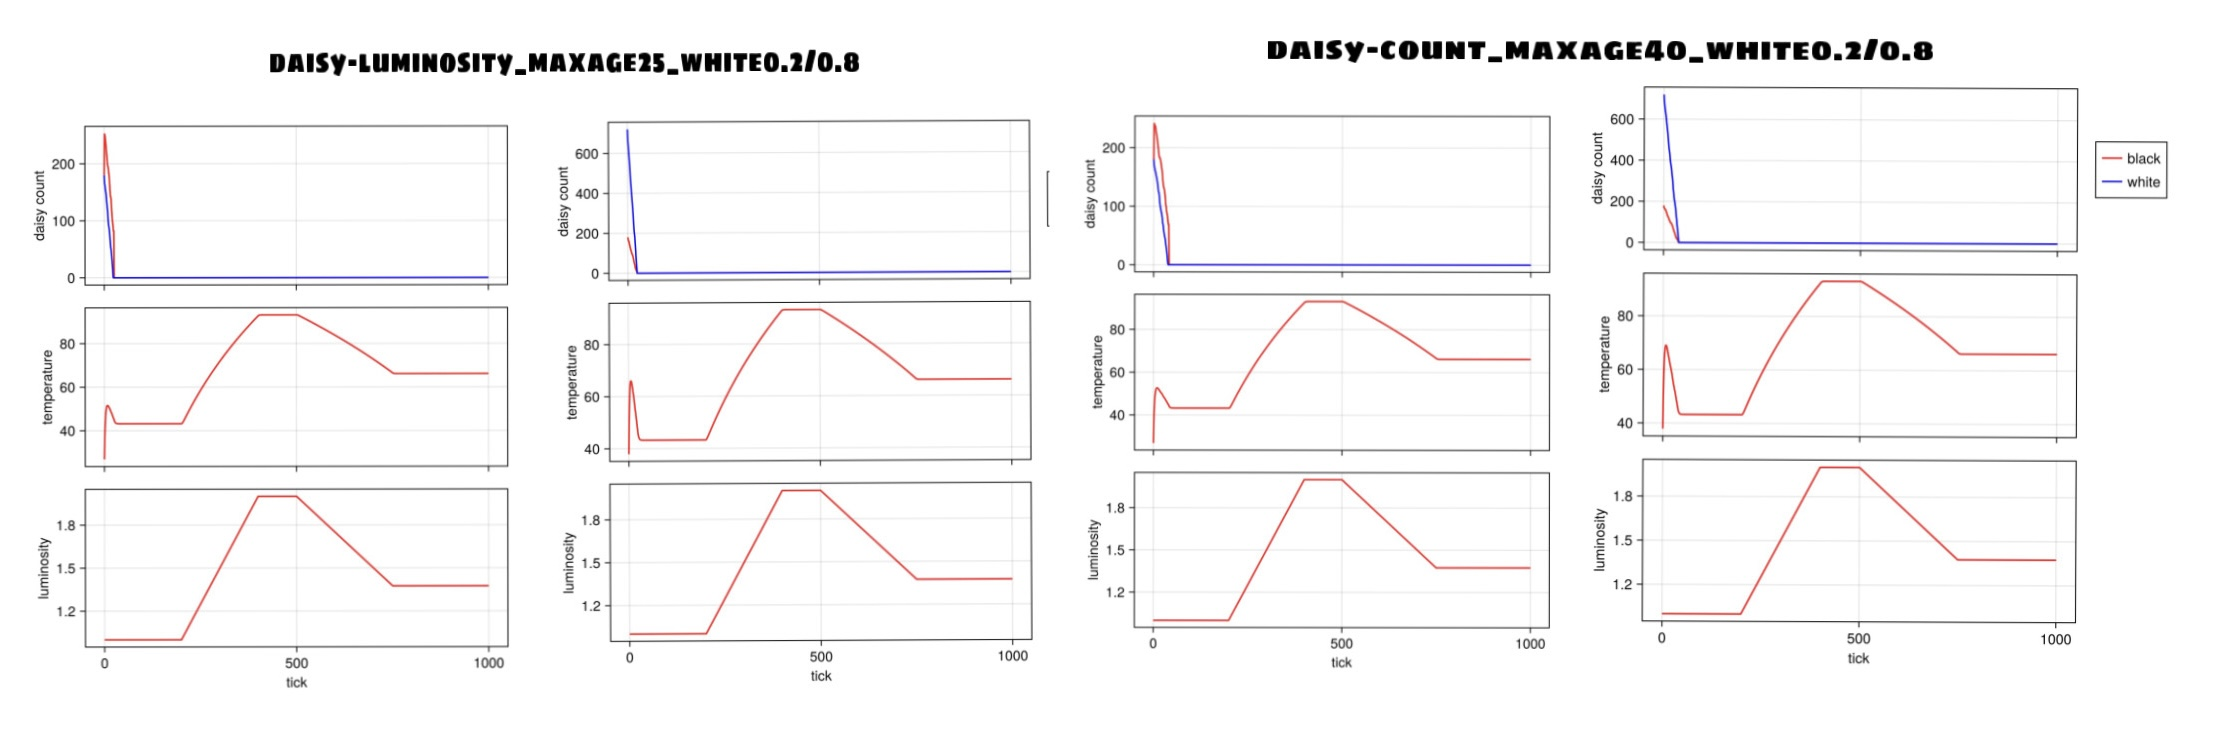
\includegraphics[width=0.7\linewidth,height=\textheight,keepaspectratio]{image/41.png}

}

\caption{\label{fig-41}графики}

\end{figure}%

\chapter{Выводы}\label{ux432ux44bux432ux43eux434ux44b}

В ходе выполнения лабораторной работы была успешно реализована и
проанализирована агентная модель Daisyworld, демонстрирующая гипотезу
Геи --- способность биоты регулировать климат планеты.


\printbibliography



\end{document}
